\subsection{Regressione}
Immaginiamo di andare in laboratorio e di raccogliere i dati di un esperimento. Quello che si è soliti fare è disporre i dati su due colonne: una raccoglie le variabili indipendenti, l'altra quelle dipendenti, che solitamente indichiamo rispettivamente con $x$ e $y$. Supponiamo quindi di avere raccolto $n+1$ dati $(x_i,y_i)$ con $i=0,\ldots,n$. Di norma gli $x_i$ sono degli scalari, ma più raramente può capitare che siano delle $p$-uple, cioè degli elementi di $\mathbb{R}^p$. Tale situazione corrisponde al caso in cui la variabile dipendente $y_i$ (che in entrambi i casi è uno scalare) dipende da diverse variabili indipendenti. Ci limiteremo al primo caso.

Ciò che di solito si fa in laboratorio è supporre di conoscere la forma funzionale $f$ della dipendenza teorica tra $y$ e $x$. In generale tale forma dipenderà da diversi parametri che indichiamo in forma vettoriale con $\underline{a}$, il quale in generale sarà una $q$-upla:

$$y=f( \underline{x};\underline{a} )$$

Il primo problema che affrontiamo in laboratorio è quello di trovare i valori più probabili\footnote{Qui e nel seguito il prof usa il termine "the most likely". Non essendo sicuro sulla traduzione più adatta a volte ho tradotto a senso.} di tali parametri che interpolano tra i dati forniti.

\vspace{0.3cm}

\begin{minipage}{0.445\textwidth}
   \centering
   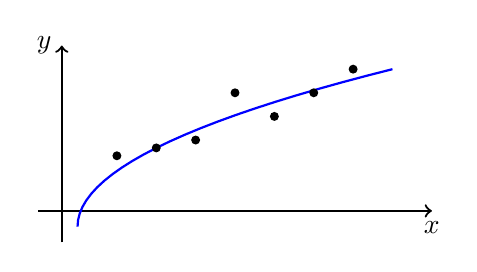
\begin{tikzpicture}[domain=0:2]
      \draw[thick,->] (-0.5,0.2) -- (4.5,0.2) node [below] {$x$};
      \draw[thick,->] (-0.2,-0.2) -- (-0.2,2.3) node [left] {$y$};
      \draw[thick,blue] plot (\x*\x,\x);
      \filldraw (0.5,0.9) circle (1.4pt);
      \filldraw (1,1) circle (1.4pt);
      \filldraw (1.5,1.1) circle (1.4pt);
      \filldraw (2,1.7) circle (1.4pt);
      \filldraw (2.5,1.4) circle (1.4pt);
      \filldraw (3,1.7) circle (1.4pt);
      \filldraw (3.5,2) circle (1.4pt);
   \end{tikzpicture}
\end{minipage}
\begin{minipage}{0.55\textwidth}
   \vspace{0.2cm}Potremmo ad esempio avere dei dati distribuiti come in figura e volerli interpolare, sapendo che la forma funzionale dovrebbe essere, ad esempio, una parabola: in questo caso essa dipenderà in generale da tre parametri.
\end{minipage}

\vspace{0.4cm}Vogliamo dunque trovare la funzione più adeguata di quel tipo di forma funzionale, la quale passa attraverso i dati nonostante non intersechi alcun punto in particolare. \E chiaro che può capitare che passi per qualcuno dei dati, ma come si evince anche dalla figura gli altri dati sono distribuiti attorno alla curva.

Da un punto di vista euristico, questa è una buona approssimazione su tutto l'insieme dei dati. In questo caso si parla di regressione, e il motivo per cui la curva è detta la più adatta è perché identifichiamo una funzione obiettivo (una funzione che vogliamo minimizzare o massimizzare, in generale ottimizzare) e andiamo a cercare i valori più adatti dei parametri $\underline{a}$ tali che la funzione è minima o massima rispetto al tipo di curva assegnata. La funzione obiettivo di cui parliamo è il $\chi^2$, la quale è definita come la differenza tra il valore misurato $y_i$ e il valore atteso $f(\underline{x}_i,\underline{a})$ elevata al quadrato:

$$\chi^2(\underline{a})
=\frac{1}{n-1} \sum_{i=0}^{n} \big[ y_i - f(\underline{x}_i,\underline{a}) \big]^2\geq0$$

Sebbene considerando il quadrato della differenza perdiamo l'informazione sul segno della differenza $y_i - f(\underline{x}_i,\underline{a})$, ciò ci permette di sapere a priori che il $\chi^2$ è una funzione non negativa, per cui è limitata dal basso: il suo minimo è 0. Inoltre, poiché tale funzione è regolare

\textbf{mi fa male la testa, continua lezione 1 14:50 circa}

$$y=f(x)=f(x_0) + f'(x_0)(x-x_0) + \frac{1}{2!}f''(x_0)(x-x_0)^2 + \ldots$$

$$\begin{cases}
   c_0 + c_1x_0 + c_2 x_0^2 + \ldots + c_n x_0^n=y_0\\
   c_0 + c_1x_1 + c_2 x_1^2 + \ldots + c_n x_1^n=y_1\\
   \vdots\\
   c_0 + c_1x_n + c_2 x_n^2 + \ldots + c_n x_n^n=y_n
\end{cases}$$

Possiamo esprimere il sistema come

$$V \underline{c}=\underline{y}$$

dove

$$V=
\begin{pmatrix}
   1 & x_0 & x_0^2 & \ldots & x_0^n\\
   1 & x_1 & x_1^2 & \ldots & x_1^n\\
   \vdots & \vdots & \vdots & \ddots & \vdots\\
   1 & x_n & x_n^2 & \ldots & x_n^n\\
\end{pmatrix}
\quad,\quad
\underline{c}=
\begin{pmatrix}
   c_0\\
   \vdots\\
   c_n
\end{pmatrix}
\quad,\quad
\underline{y}=
\begin{pmatrix}
   y_0\\
   \vdots\\
   y_n
\end{pmatrix}$$

$V$ è detta \textbf{matrice di Vandermonde}. Poiché $x_i \neq x_j \quad \forall \, i \neq j$, ogni colonna è diversa e quindi il determinante è non nullo. Per calcolarlo sottraiamo ad ogni colonna la precedente moltiplicata per $x_0$:

$$\det (V)=
\begin{pmatrix}
   1 & x_0 - x_0 & x_0^2 - x_0^2 & \ldots & x_0^n - x_0^n\\
   1 & x_1 - x_0 & x_1^2 - x_0x_1 & \ldots & x_1^n - x_0x_1^{n-1}\\
   \vdots & \vdots & \vdots & \ddots & \vdots\\
   1 & x_n - x_0 & x_n^2 - x_0x_n & \ldots & x_n^n - x_0 x_n^{n-1}\\
\end{pmatrix}$$

$$\implies \det (V)=
\begin{pmatrix}
   1 & 0 & 0 & \ldots & 0\\
   1 & x_1 - x_0 & (x_1 - x_0)x_1 & \ldots & (x_1 - x_0)x_1^{n-1}\\
   \vdots & \vdots & \vdots & \ddots & \vdots\\
   1 & x_n - x_0 & (x_n - x_0)x_n & \ldots & (x_n - x_0)x_n^{n-1}\\
\end{pmatrix}$$

dividendo la $j$-esima riga (tranne la prima) per $x_j - x_0$ e portando fuori dalla matrice otteniamo

$$\det (V)=
\begin{pmatrix}
   1 & 0 & 0 & \ldots & 0\\
   1 & 1 & x_1 & \ldots & x_1^{n-1}\\
   \vdots & \vdots & \vdots & \ddots & \vdots\\
   1 & 1 & x_n & \ldots & x_n^{n-1}\\
\end{pmatrix}
\underbrace{(x_1 - x_0) \cdot \ldots \cdot (x_n - x_0)}_{\displaystyle = \prod_{j=2}^{n} (x_j - x_0)}$$

La matrice risultante non dipende più da $x_0$. Reiterando il processo possiamo eliminare la dipendenza da ogni $x_i$ e in forma compatta il determinante si potrà scrivere come

$$\det V=\prod_{i>j} (x_i - x_j)$$

Tale espressione ci dice che se i punti sono tutti distinti il determinante della matrice è diverso da zero. Si può anche scrivere come

$$\det V=\prod_{j=0}^{n-1} \qty( \prod_{i=j+1}^{n} (x_i - x_j) )$$

\textbf{non ho capito come si passa a questo vabbè}

$$P_n(x)=\sum_{i=0}^{n} f(x_i) L_i(x)$$

dove

$$L_i(x)=\prod_{\begin{subarray}{c}
   k=0\\[0.1cm]
   k \neq i
\end{subarray}
}^{n} \frac{x - x_k}{x_i - x_k}
$$

nota: essendo così definito, il denominatore è sempre diverso da zero.

L'ordine di ogni polinomio $L_i$ è proprio $n$

$$L_i=\frac{
(x - x_0) (x - x_1) \ldots (x - x_{i-1}) (x - x_{i+1}) \ldots (x - x_n)
}{
(x_i - x_0) (x_i - x_1) \ldots (x_i - x_{i-1}) (x_i - x_{i+1}) \ldots (x_i - x_n)
}$$

Si ha che

$$L_i(x_j)=
\left\{
   \begin{array}{ll}
      0 & \text{se } j \neq i\\
      1 & \text{se } j = i
   \end{array}
\right.
\equiv \delta_{ij}$$

infatti nel primo caso a numeratore ci sarà un termine nullo, nel secondo caso numeratore e denominatore saranno uguali.

In definitiva abbiamo che

$$P_n(x_j)=\sum_{i=0}^{n} f(x_i) L_i(x_j)
=\sum_{i=0}^{n} f(x_i) \delta_{ij}
=f(x_j) \quad \forall \, j$$

\subsection{Formula di Newton per il polinomio interpolante}

Tale metodo si adopera quando abbiamo trovato la soluzione per $n$ punti e ne includiamo un altro. Supposto quindi di avere il polinomio $P_{n-1}(x)$ che passa per $x_0,x_1,\ldots,x_{n-1}$, poniamo

$$P_n(x)=P_{n-1}(x) + a_n w_{n-1}(x)$$

dove

$$w_{n-1}(x)=\prod_{i=0}^{n-1} (x - x_i)
\quad,\quad
a_n=\frac{f(x_n) - P_{n-1}(x_n)}{w_{n-1}(x_n)}$$

$w_{n-1}$ è un \textit{polinomio monico}, cioè un polinomio tale che il coefficiente del termine di grado massimo è pari a 1. Inoltre ha grado $n$.

\vspace{0.2cm}Proviamo innanzitutto che il nuovo polinomio passa per i primi $n-1$ punti.

Posto $k \leq n-1$ si ha

$$w_{n-1}(x_k)=0$$
$$P_n(x_k)=P_{n-1}(x_k) + a_n \underbrace{w_{n-1}(x_k)}_{=0}
=P_{n-1}(x_k)
\equiv f(x_k)$$

Proviamo adesso che passa per il nuovo punto:

$$P_n(x_n)=P_{n-1}(x_n) + a_n w_{n-1}(x_n)
=P_{n-1}(x_n) + \frac{f(x_n) - P_{n-1}(x_n)}{w_{n-1}(x_n)} w_{n-1}(x_n)=$$
$$=P_{n-1}(x_n) + f(x_n) - P_{n-1}(x_n)
=f(x_n) $$

$$P_n(x)=c_0 + c_1x + c_2x^2 + \ldots + c_nx^n=$$
$$=c_0 + a_1(x-x_0) + a_2(x-x_0)(x-x_1) + \ldots + a_n(x-x_0)(x-x_1)\ldots(x-x_n)=$$
$$=\sum_{k=0}^{n} a_k w_{k-1}(x)$$

\section{Errore nell'estrapolazione}

$$w_n(x)=F(x)=\prod_{k=0}^{n} (x - x_k)
\quad,\quad
F_i(x)=\prod_{
   \begin{subarray}{c}
      k=0\\[0.1cm]
      k \neq 1
   \end{subarray}
}^{n} (x - x_k)$$

Sia $\overline{x} \neq x_k$ (tra i nodi) tale che $\displaystyle a \leq \min_{k} x_k < \overline{x} < \max_{k} x_k \leq b$.

Sia

$$G(x)=f(x) - P_n(x) - RF(x)$$

dove $R$ è un parametro scelto in maniera tale che $G(\overline{x})=0$. $G$ è uguale all'errore ma corretto con $F(x)$. Si ha che

$$G(x_k)=f(x_k) - P_n(x_k) - RF(x_k)=0
\quad \forall \, x_k \;,\; k=0,1,\ldots,n$$

perché è una nodal function. Ne segue che $G(x)$ si annulla in $n+2$ punti: $x_0,x_1,\ldots,\overline{x},\ldots,x_n$. Per il teorema di Rolle, $G'(x)$ si annullerà in $n+1$ punti intermedi. Reiterando tale teorema otteniamo che $G^{(n+1)}(x)$ si annullerà in un solo punto $\xi \in [a,b]$. D'altra parte:

\begin{itemize}
   \item $P_n(x)$ è un polinomio di grado minore o uguale $n$, per cui $P^{(n+1)}=0$;
   \item $F(x)$ è un polinomio monico di grado $n+1$, dunque $F^{(n+1)}(x)=(n+1)!$
\end{itemize}

In definitiva:

$$G^{(n+1)}(x)=f^{(n+1)}(x) + 0 - R(n+1)!$$

Abbiamo visto che

$$\exists \, \xi : G^{(n+1)}(\xi)=f^{(n+1)}(\xi) - R(n+1)!=0
\implies
R=\frac{f^{(n+1)}(\xi)}{R(n+1)!}$$

$$\implies G(x)=f(x) - P_n(x) - \eval{\frac{f^{(n+1)}(\xi)}{(n+1)!} F(x)}_{x=\overline{x}}=0$$

$$f(x)=P_n(x) + \frac{f^{(n+1)}(\xi)}{(n+1)!} w_n(x)$$

\subsection{Prodotto scalare (prodotto hermitiano)}

Applicazione lineare $\braket*{\, \cdot \, }{\, \cdot \,}:V \times V \to \mathbb{C}$

\begin{enumerate}[label=(\roman*)]
   \item $\braket*{u}{v}=\braket*{v}{u}^*$
   \item $\braket*{u}{\lambda_1 v_1 + \lambda_2 v_2}=\lambda_21\braket*{u}{v_1} + \lambda_2 \braket*{u}{v_2}$
   
   $\braket*{\lambda_1 u_1 + \lambda_2 u_2}{v}=\lambda^*_2 \braket*{u_1}{v} + \lambda^*_2 \braket*{u_2}{v}$
   \item $\braket*{u}{u} \geq 0$, $\braket*{u}{u}=0 \iff u=0$
\end{enumerate}

\subsection{Polinomi di Legendre}

$$\braket*{\phi_k}{\phi_{k'}}c_{k'}
=\braket*{\phi_k}{v}$$

$$\begin{pmatrix}
   \braket*{\phi_0}{\phi_0} & \braket*{\phi_0}{\phi_1} & \ldots & \braket*{\phi_0}{\phi_n}\\
   \vdots &\vdots & \ddots & \vdots\\
   \braket*{\phi_n}{\phi_0} & \ldots & \ldots & \braket*{\phi_n}{\phi_n}
\end{pmatrix}
\begin{pmatrix}
   c_0\\
   \vdots\\
   c_n
\end{pmatrix}
=
\begin{pmatrix}
   \braket*{\phi_0}{v}\\
   \vdots\\
   \braket*{\phi_n}{v}
\end{pmatrix}$$

$$\| \phi_0 \|^2
=\braket*{\phi_0}{\phi_0}
=\int_{-1}^{1} 1 \cdot 1 \dd{x}=2
\implies
\tilde{P}(x)=\frac{1}{\sqrt{2}}$$

Dunque il primo polinomio di Legendre è ancora una costante.

$$\tilde{P}_1=\phi_1 - \hat{P}_0 \braket*{\hat{P}_0}{\phi_1}=\phi_1=x$$

$$\braket*{\hat{P}_0}{\phi_1}=\int_{-1}^{1} \frac{1}{\sqrt{2}} x \dd{x}=0$$

(perché l'integranda è dispari e l'intervallo è simmetrico)

$$\implies \hat{P}_1
=\frac{x}{\displaystyle \sqrt{\frac{2}{3}}}
=\sqrt{\frac{3}{2}}x$$

$$
\begin{array}{lcccc}
   k && p_k(x) \text{ (ortogonali)} && \hat{p}_k(x) \text{ (ortonormali)}\\[0.2cm]
   0 && 1 && \displaystyle \sqrt{\frac{1}{2}}\\[0.4cm]
   1 && x && \displaystyle x \sqrt{\frac{3}{2}}\\[0.4cm]
   2 && \displaystyle \frac{3x^2 - 1}{2} && \displaystyle \frac{3x^2 - 1}{2} \sqrt{\frac{5}{2}}\\[0.4cm]
   3 && \displaystyle \frac{5x^3 - 3x^2}{2} && \displaystyle \frac{5x^3 - 3x^2}{2} \sqrt{\frac{7}{2}}\\[0.4cm]
   4 && \displaystyle \frac{35x^4 - 30 x^2 + 2}{8} && \displaystyle \frac{35x^4 - 30 x^2 + 2}{8} \sqrt{\frac{9}{2}}\\[0.4cm]
\end{array}$$

\subsubsection{Sviluppo in multipolo}

$$V(\underline{r})=\frac{1}{4 \pi \varepsilon_0} \int_{\Omega} \frac{\rho(\underline{r}')}{| \underline{r} - \underline{r}' |} \dd[3]{\underline{r}'}$$

$$Q=\int_{\Omega} \rho(\underline{r}') \dd[3]\underline{r}'$$

Il potenziale allora sarà

$$V(\underline{r}) \approxeq \frac{1}{4 \pi \varepsilon_0}\frac{Q}{r}$$

$$\frac{1}{| \underline{r} - \underline{r}' |}
=\frac{1}{\sqrt{r^2 + r'^2 - 2 r r' \cos{\vartheta}}}$$

$$r_{>}=\max \qty{r,r'}
\quad,\quad
r_{<}=\min \qty{r,r'}$$

Supponiamo che $\underline{r} \neq \underline{r}' \iff \underline{r} - \underline{r}' \neq 0$

$$\frac{1}{| \underline{r} - \underline{r}' |}
=\frac{1}{r_{>} \displaystyle \sqrt{1 - 2\frac{r_{<}}{r_{>}} \cos{\vartheta} + \qty(\frac{r_{<}}{r_{>}})^2}}$$

Consideriamo l'espansione di Taylor

$$\frac{1}{\sqrt{1 + x}}=1 - \frac{1}{2}x + \frac{1 \cdot 3}{2 \cdot 4} x^2 - \frac{1 \cdot 3 \cdot 5}{2 \cdot 4 \cdot 6} x^3
\quad \text{per } |x|<1$$

Se poniamo

$$x=- 2\frac{r_{<}}{r_{>}} \cos{\vartheta} + \qty(\frac{r_{<}}{r_{>}})^2$$

\subsection{Funzione generatrice per polinomi ortonormali}

Siano $\qty{P_n}$ un insieme di polinomi ortogonali e normalizzati rispetto ad un peso dato \textbf{sta parte mi sembra poco chiara}

Si avrà

$$\delta_{nm}=\braket*{P_n}{P_m}
=\int_{a}^{b} P_n(x) P_m(x) w(x) \dd{x}$$

$$\braket*{Q_{n-1}}{P_n}
=\int_{a}^{b} P_n(x) Q_{n-1}(x) w(x) \dd{x}=0$$

$$U_n(x): \quad w(x) P_n(x)=\dv[n]{U_n(x)}{x}$$

$$\int_{a}^{b} Q_{n-1}(x) w(x) P_n(x) \dd{x}=0$$

$$0=\int_{a}^{b} Q_{n-1}(x) \dv[n]{U_n(x)}{x} \dd{x}$$

Tale integrale può essere risolto integrando per parti $n$ volte. La prima volta si ha

$$=\qty[Q_{n-1}(x) \dv[n-1]{U_n(x)}{x}]_{a}^{b}
- \int_{a}^{b} Q'_{n-1}(x) \dv[n-1]{U_n(x)}{x} \dd{x}$$

($Q'_{n-1}(x)$ ha grado $n-2$). Reiterando il processo si ha

$$=\Big[ Q_{n-1}(x) U_n^{(n-1)}(x) - Q'_{n-1}(x) U_n^{(n-2)}(x) + $$
$$+Q''_{n-1}(x) U_n^{(n-3)}(x) + \ldots + (-1)^{n-1} Q^{(n-1)}_{n-1}(x) U_n(x) \Big]_{a}^{b}$$

$$\begin{cases}
   U_n(a)=U_n'(a)=\ldots=U_n^{(n-1)}(a)=0\\[0.1cm]
   U_n(b)=U_n'(b)=\ldots=U_n^{(n-1)}(b)=0\\
\end{cases}$$

$$P_n(x)=\frac{1}{w(x)} \dv[n]{U_n(x)}{x}$$

(Si può fare perché $w>0 \quad \forall \, x \in [a,b]$)

Tale espressione è un polinomio di grado $n$, che se viene differenziato $n+1$ volte diventa 0:

$$P_n^{(n+1)}=0$$

Segue che

$$\dv[n+1]{x} \qty[ \frac{1}{w(x)} \dv[n]{U_n(x)}{x} ]=0$$

$$\dv[2n+1]{x} U_n(x)=0$$

$$\begin{cases}
   U_n(-1)=U_n'(-1)=\ldots=U_n^{(n-1)}(-1)=0\\[0.1cm]
   U_n(1)=U_n'(1)=\ldots=U_n^{(n-1)}(1)=0\\
\end{cases}$$

$$U_n(x)=c_n (x^2 - 1)^n$$

$$P_n(x)=c_n \dv[n]{x} (x^2 - 1)^n
=c_n \dv[n]{x} \big[ (x + 1)^n (x - 1)^n \big]=$$
$$=c_n \qty[ (x+1)^n \dv[n]{x} (x - 1)^n + n \dv{x} (x+1)^n \dv[n-1]{x} (x-1)^n + \ldots]$$

Si ha che

$$\dv[n]{x} \eval{(x-1)^n}_{x=1}
=\dv[n]{x} \eval{(x^n + \ldots )}_{x=1}=n!$$

(solo il primo termine termine sopravvive, diventando una costante pari a $n!$)

per gli altri termini invece si ha

$$\dv[n-k]{x} \eval{(x-1)^n}_{x=1}=0 \quad \forall \, k>2$$

Dunque

$$P_n(1)=c_n 2^n n! + 0$$

Se imponiamo la condizione $P_n(1)=1$ si ottiene

$$c_n 2^n n!=1
\implies
c_n=\frac{1}{ 2^n n! }$$

Allora il generico polinomio di Legendre sarà definito come

$$P_n(x)=\frac{2}{ 2^n n! } \dv[n]{x} (x^2 - 1)^n$$

\subsection{Formule ricorsive}

Esse sono formule che permettono di trovare un polinomio in un certo punto $x$ avendo alcuni polinomi calcolati nello stesso punto ma con indice minore (ad esempio per trovare $P_n$ ci serve $P_{n-1}$ e $P_{n-2}$). Quindi piuttosto che derivare diverse volte la funzione generatrice si può partire da alcuni polinomi e combinarli per ottenere i successivi.

Per ottenere la formula si parte dall'identità

$$\phi(t,x)=\frac{1}{\sqrt{1 - 2xt + t^2}}$$

Essa è simile a

$$\frac{1}{| \underline{r} - \underline{r}' |}
=\frac{1}{r_{>} \displaystyle \sqrt{1 - 2\frac{r_{<}}{r_{>}} \cos{\vartheta} + \qty(\frac{r_{<}}{r_{>}})^2}}
\quad\text{con}\quad
\begin{cases}
   \displaystyle t=\frac{r_{<}}{r_{>}}\\[0.4cm]
   \cos{\vartheta}=x
\end{cases}$$

di cui abbiamo ricavato l'espansione in multipolo. Essa sarà:

$$\phi(t,x)=\sum_{l=0}^{\infty} P_l(x) t^l$$

$$\pdv{\phi}{t}
=-\frac{1}{2} \frac{-2x+2t}{(1-2xt+t^2)^{\frac{3}{2}}}
=\phi(t,x) \frac{x - t}{1-2xt+t^2}
=\frac{x - t}{1-2xt+t^2} \sum_{l=0}^{\infty} P_l(x) t^l$$

$$\pdv{t} \sum_{l=0}^{\infty} P_l(x) t^l
=\sum_{l=0}^{\infty} P_l(x) l t^{l - 1}$$

Le derivate dei due termini devono essere uguali, quindi:

$$\sum_{l=0}^{\infty} l P_l(x) t^{l - 1}
=\frac{x-t}{1 - 2xt + t^2} \sum_{l=0}^{\infty} P_l(x) t^l$$

Per poter scrivere tutto come un unico polinomio in $t$ e porre i coefficienti di tale polinomio uguali a zero (principio di identità dei polinomi) moltiplichiamo entrambi i termini per $(1 - 2xt + t^2)$:

$$(1 - 2xt + t^2)\sum_{l=0}^{\infty} l P_l(x) t^{l - 1}
=(x - t) \sum_{l=0}^{\infty} P_l(x) t^l$$

Nella sommatoria del primo membro, il termine per $l=0$ è nullo, quindi possiamo partire da $l=1$. Per partire comunque da $l=0$ scriviamo

$$(1 - 2xt + t^2)\sum_{l=0}^{\infty} (l + 1) P_{l + 1}(x) t^{l +1 - 1}
=(x - t) \sum_{l=0}^{\infty} P_l(x) t^l$$

cioè a sinistra partiamo da $l+1$ anziché da $l$. Avendo due sommatorie simili possiamo raggrupparle e, moltiplicando per i rispettivi fattori davanti alle sommatorie, si ha

$$\sum_{l=0}^{\infty} \big[ (l + 1)P_{l + 1}(x) t^l - 2(l + 1)x P_{l + 1}(x) t^{l+1} +$$
$$+ (l + 1)P_{l+1}(x)t^{l+2} - x P_l(x)t^l + P_l(x)t^{l+1} \big]=0
\quad \forall \, x,t$$

Raggruppiamo i termini con la potenza di $t$:

$$\sum_{l=0}^{\infty} \Big\{ \big[ (l+1)P_{l+1}(x) - xP_l(x) \big] t^l + \big[ P_l(x) -2(l+1)xP_{l+1}(x) \big]t^{l+1} + (l+1)P_{l+1}(x)t^{l+2} \Big\}=0$$

\subsection{Approssimazione di integrali}

$$f(x)=y_k + \frac{y_{k+1} - y_k}{x_{k+1} - x_k} (x - x_k)
=y_k + \underbrace{\frac{y_{k+1} - y_k}{h}}_{\approx f'_k + o(h)} (x - x_k)$$

$$\int_{x_k}^{x_{k+1}} f(x) \dd{x}
=\int_{x_k}^{x_{k+1}} \qty{ y_k + \Big( \frac{y_{k+1} - y_k}{h} + o(h) \Big)(x - x_k) } \dd{x}=$$
$$=y_k(x_{k+1} - x_k) + \qty[ \frac{y_{k+1} - y_k}{h} + o(h) ]\qty[ \frac{(x - x_k)^2}{2} ]_{x_k}^{x_{k+1}}$$

\subsection{Il modello di Ising}

Il modello di Ising è un modello per il magnetismo nato per spiegare la transizione da una fase magnetica all'altra passando da un regime a temperatura più bassa ad uno a temperatura più alta in cui molti spin, molti momenti magnetici si orientano nella stessa direzione. Sia $i$ un nodo e $S_i$ il relativo spin. Ising fece un modello monodimensionale in cui abbiamo una sola linea con i nodi isolati, e ogni relativo spin si assume possa essere diretto solo verso l'alto o verso il basso ($+1$ e $-1$)

\begin{center}
   \begin{tikzpicture}[scale=1.5]
      \draw (-2,0) -- (2,0);
      \draw[thick,->] (-0.5,-0.2) -- (-0.5,0.2);
      \draw[thick,->] (0.5,0.2) -- (0.5,-0.2);
      \node at (4,0) {$S_i \in \qty{+1,-1}$};
   \end{tikzpicture}
\end{center}

Gli spin interagiscono tra loro, ma per semplicità assumiamo che possono interagire solo due spin tra loro vicini.

L'energia del sistema può crescere o decrescere a seconda che il loro prodotto sia positivo o negativo.

L'hamiltoniana del sistema per l'energia si scrive come

$$\mathcal{H}=\sum_{\expval{ij}} J_{ij} S_i S_j
\quad\text{dove}\quad
J_{ij}=\left\{
   \begin{array}{lc}
      +J & \rm AFM\\
      -J & \rm FM
   \end{array}
\right.$$

La scrittura $\expval*{ij}$ indica che consideriamo soltanto l'interazione tra spazi vicini. I due valori di $J_{ij}$ rappresentano un sistema ferromagnetico (FM) e uno anti-ferromagnetico (AFM), cioè quando gli spin sono paralleli (entrambi +1 o entrambi -1)

$$\mathcal{H}=\sum_{\expval{ij}} J_{ij} S_i S_j - H \sum_{i} S_i$$

$$m=\frac{1}{N} \sum_{i} S_i$$

$$\expval*{o}=\frac{1}{z} \sum_{S} o(S) e^{-\frac{H(S)}{k_b T}}$$